
El aprendizaje por refuerzo (RL, por sus siglas en inglés) constituye un paradigma de la inteligencia artificial
que permite a un agente aprender a tomar decisiones óptimas mediante la interacción con un entorno.
A diferencia del aprendizaje supervisado, donde se dispone de ejemplos etiquetados, o del no supervisado,
que busca patrones ocultos, el aprendizaje por refuerzo se basa en un proceso de prueba y error donde el agente
recibe retroalimentación en forma de recompensas o penalizaciones según las consecuencias de sus acciones.


La IA puede contribuir significativamente a la mejora de los sistemas de asistencia al conductor.
Si una IA aprendiera a estacionar un vehículo en un ambiente controlado, este conocimiento podría
proporcionar información valiosa para automatizar esta tarea compleja. Los algoritmos de aprendizaje
por refuerzo son candidatos naturales para este tipo de problemas secuenciales de toma de decisiones.

\subsection{Componentes fundamentales del aprendizaje por refuerzo}\label{subsec:rl-components}

El framework de aprendizaje por refuerzo se estructura alrededor de la interacción cíclica entre
cuatro elementos principales representados en la figura \ref{fig:rl-cycle}:

\begin{figure}[!ht]
    \centering
    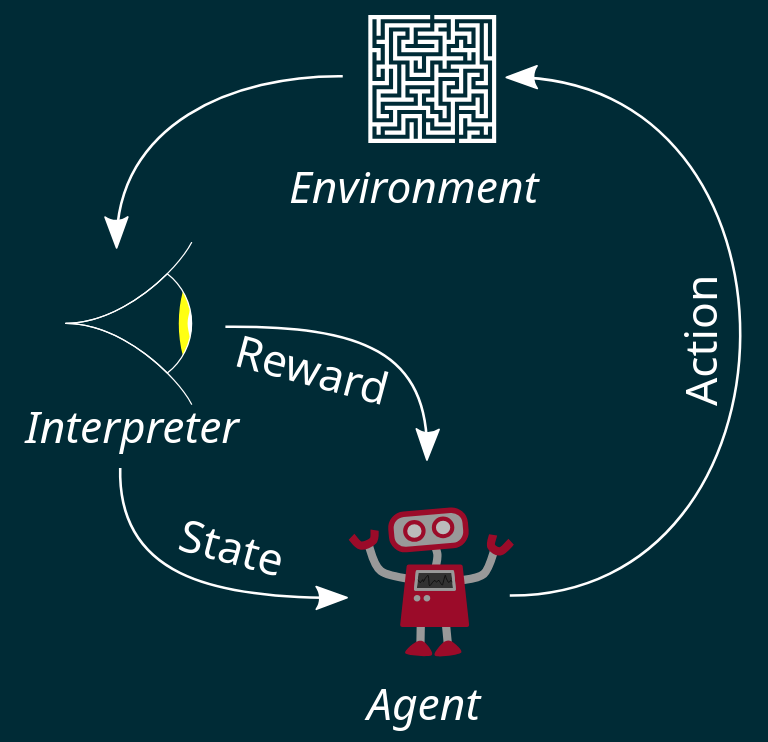
\includegraphics[width=0.5\textwidth]{img/2-mt/RL.png}
    \caption{Ciclo básico del aprendizaje por refuerzo: interacción agente-entorno.}
    \label{fig:rl-cycle}
\end{figure}

\begin{itemize}
    \item \textbf{Agente}: entidad que toma decisiones y ejecuta acciones. En el contexto de estacionamiento automático,
    el agente corresponde al sistema de control del vehículo que decide las maniobras a realizar.
    
    \item \textbf{Entorno}: sistema o mundo en el que opera el agente. Para estacionamiento, incluye
    el espacio físico del estacionamiento, otros vehículos, obstáculos y las leyes físicas que gobiernan
    el movimiento vehicular.
    
    \item \textbf{Estado}: representación de la situación actual del sistema. Típicamente incluye
    información sobre la posición, orientación y velocidad del vehículo, así como la disposición
    del entorno circundante.
    
    \item \textbf{Acción}: decisión o maniobra que el agente puede ejecutar para cambiar el estado
    del entorno. En conducción, las acciones básicas incluyen acelerar, frenar y girar el volante.
    
    \item \textbf{Recompensa}: señal numérica que evalúa qué tan buena o mala fue una acción particular
    en un estado dado. Una función de recompensa bien diseñada guía al agente hacia comportamientos deseables
    (como estacionar correctamente) y penaliza acciones indeseables (como colisiones).
    
    \item \textbf{Política}: estrategia que determina qué acción tomar en cada estado. El objetivo
    del aprendizaje por refuerzo es encontrar una política óptima que maximice la recompensa acumulada.
\end{itemize}

\subsection{Aplicación al estacionamiento automático}\label{subsec:rl-parking}

En el problema de estacionamiento automático, el agente (vehículo) debe aprender a navegar desde
una posición inicial hasta un cajón de estacionamiento objetivo, evitando obstáculos y respetando
las limitaciones físicas del vehículo. El estado puede incluir la pose del vehículo (posición y orientación)
relativa al objetivo, mientras que las acciones corresponden a comandos de aceleración y dirección.


La recompensa típicamente incorpora múltiples criterios: proximidad al objetivo, penalizaciones por colisiones,
suavidad de la trayectoria, y cumplimiento de restricciones geométricas del estacionamiento.
Un intérprete basado en sensores (como el sistema de visión desarrollado en este trabajo) proporciona
la información de estado necesaria para que el agente tome decisiones informadas.


Esta aproximación permite que el sistema aprenda estrategias de estacionamiento sin programación explícita
de todas las situaciones posibles, adaptándose a diferentes configuraciones de estacionamiento y
condiciones del entorno a través de la experiencia acumulada durante el entrenamiento.
